% TODO: Put shorting in the start of the timeline (t_0)
\usetikzlibrary{calc, arrows.meta, intersections, patterns, positioning, shapes.misc, fadings, through,decorations.pathreplacing}

\begin{figure}[t]
\centering
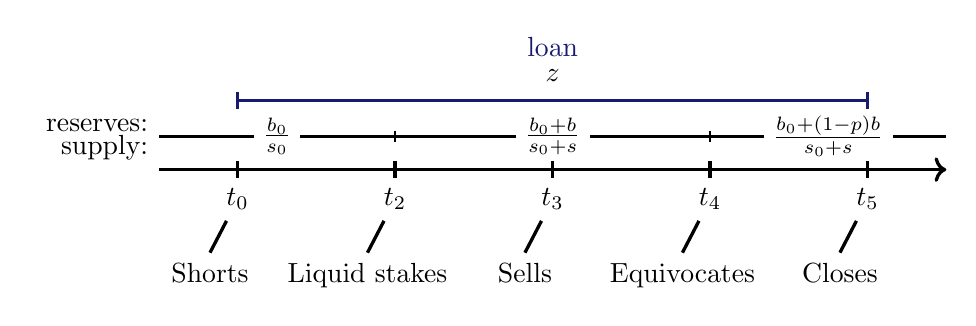
\begin{tikzpicture}[very thick, black]

\coordinate (distance) at (2,0);

\coordinate (O) at (-1,0); % Origin
\coordinate (P0) at (0,0);
\coordinate (P2) at ($(P0) + (distance)$);
\coordinate (P3) at ($(P2) + (distance)$);
\coordinate (P4) at ($(P3) + (distance)$);
\coordinate (P5) at ($(P4) + (distance)$);
\coordinate (F) at (9,0); %End

\node[anchor=east,yshift=16pt] at (O) {{\tiny \asset} reserves:};
\node[anchor=east,yshift=8pt] at (O) {{\tiny \stasset} supply:};

\coordinate[above=12pt] (M0) at (O);
\coordinate[above=12pt] (M1) at (P2);
\coordinate[above=12pt] (M2) at (P4);
\coordinate[above=12pt] (M3) at (F);

\draw[line width=0.8pt] (M0) -- (M1) node[color=black,midway,fill=white] {$\frac{b_0}{s_0}$};
\draw[line width=0.8pt] (M2) -- (M3) node[color=black,midway,fill=white] {$\frac{\textcolor{BrickRed}{\blacktriangledown} b_0 + (1 - p) b}{s_0 + s}$};

\draw[line width=0.8pt] ($(M1) + (0,2pt)$) -- ($(M1) + (0,-2pt)$);
\draw[line width=0.8pt] ($(M2) + (0,2pt)$) -- ($(M2) + (0,-2pt)$);
\draw[line width=0.8pt] (M1) -- (M2) node[color=black,midway, fill=white] {$\frac{\textcolor{PineGreen}{\blacktriangle} b_0 + b}{\textcolor{PineGreen}{\blacktriangle} s_0 + s}$};


%% Timeline
\draw[->] (O) -- (F);


%% Ticks
\foreach \x in {P0,P2,P3,P4,P5}
\draw ($(\x) - (0,3pt)$) -- ($(\x) + (0,3pt)$);


%% t_1
\draw (P0) node[below=3pt](T0) {$t_0$} ;
\node[below=30pt,xshift=-10pt](D0) at (P0) {%
	Shorts};
\draw (T0) --  (D0.north);

%% t_2
\draw (P2) node[below=3pt](T2) {$t_2$} ;
\node[below=30pt,xshift=-10pt](D2) at (P2) {%
	Liquid stakes};
\draw (T2) --  (D2.north);

%% t_3
\draw (P3) node[below=3pt](T3) {$t_3$} ;
\node[below=30pt,xshift=-10pt](D3) at (P3) {%
	Sells};
\draw (T3) --  (D3.north);

%% t_4
\draw (P4) node[below=3pt](T4) {$t_4$} ;
\node[below=30pt,xshift=-10pt](D4) at (P4) {%
  Equivocates};
\draw (T4) --  (D4.north);

%% t_5
\draw (P5) node[below=3pt](T5) {$t_5$} ;
\node[below=30pt,xshift=-10pt](D5) at (P5) {%
  Closes};
\draw (T5) --  (D5.north);


%% Loans
\coordinate[above=25pt] (R0) at (P0);
\coordinate[above=25pt] (R5) at (P5);


\draw[color=MidnightBlue] ($(R0) + (0,3pt)$) -- ($(R0) + (0,-3pt)$);
\draw[color=MidnightBlue] ($(R5) + (0,3pt)$) -- ($(R5) + (0,-3pt)$);
\draw[color=MidnightBlue] (R0) -- (R5) node[color=black,midway, above=3pt](L) {$z$ {\tiny \stasset}};
\node[text=MidnightBlue,above=3pt] at (L) {loan};

\end{tikzpicture}

\caption{Timeline of the profitable attack.}
\label{fig:timeline}
\end{figure}
